% Chương 3: Kết quả thực hiện

\chapter{Kết quả thực hiện}

\section{Kiến trúc tổng thể hệ thống}

Hệ thống phát hiện xu hướng xã hội được xây dựng theo kiến trúc ba tầng: tầng thu thập dữ liệu (Producer), tầng xử lý phân tích (Consumer), và tầng giao diện người dùng (Dashboard). Luồng dữ liệu chạy một chiều từ các nguồn mạng xã hội, qua Apache Kafka message queue, đến pipeline xử lý PySpark, cuối cùng lưu vào MongoDB và hiển thị trên Streamlit dashboard.

Tầng Producer sử dụng các API và công cụ scraping để thu thập dữ liệu từ ba nguồn TikTok, YouTube và News, sau đó gửi vào ba Kafka topics tương ứng (tiktok-raw, youtube-raw, news-raw). Tầng Consumer đọc dữ liệu từ Kafka, xử lý qua pipeline tám giai đoạn sử dụng PySpark, và lưu kết quả vào MongoDB. Tầng Dashboard sử dụng Streamlit để cung cấp hai giao diện: user dashboard cho người dùng xem xu hướng và admin dashboard cho quản trị viên quản lý hệ thống.

Hệ thống hoạt động theo chế độ batch với chu kỳ bốn giờ một lần. Mỗi lần chạy, Producer thu thập khoảng 1500-2000 nội dung mới, Consumer xử lý và phát hiện các cụm xu hướng, sau đó cập nhật vào database. Dashboard tự động làm mới để hiển thị xu hướng mới nhất. Toàn bộ hệ thống được đóng gói bằng Docker để đảm bảo tính nhất quán giữa các môi trường.

\begin{figure}[H]
    \centering
    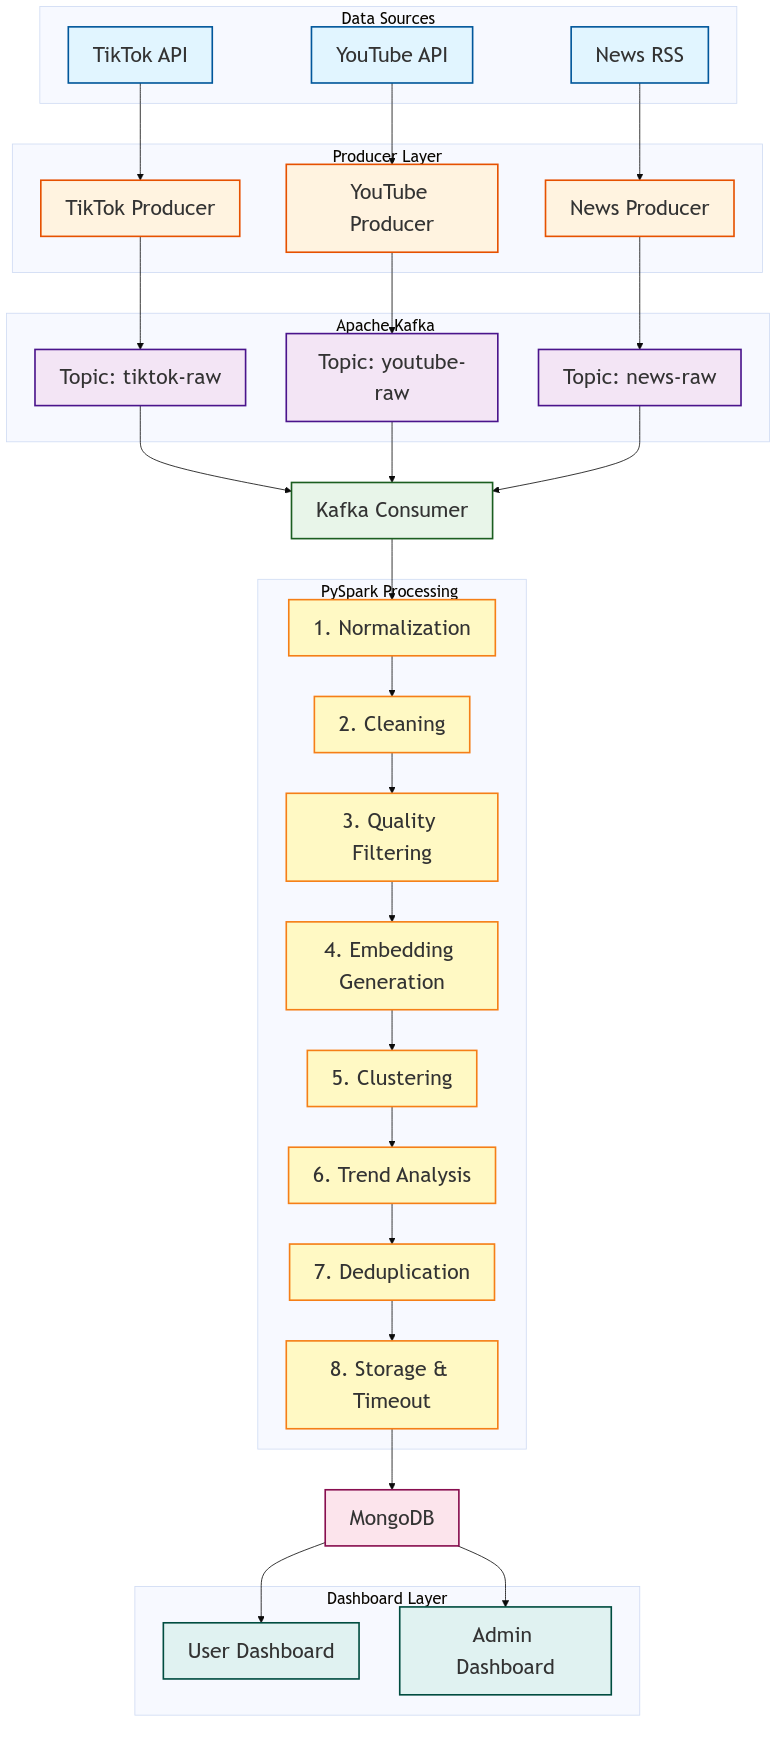
\includegraphics[width=0.6\textwidth]{images/architecture.png}
    \caption{Sơ đồ kiến trúc tổng thể hệ thống phát hiện xu hướng xã hội}
    \label{fig:architecture}
\end{figure}

\section{Tầng thu thập dữ liệu (Producer)}

\subsection{Thu thập từ TikTok}

Producer TikTok sử dụng Apify API để thu thập video từ các hashtag hoặc từ khóa đang theo dõi. Mỗi lần chạy, hệ thống lấy 100 video mới nhất cho mỗi từ khóa, tổng cộng khoảng 300-500 video tùy thuộc vào số lượng từ khóa active. Dữ liệu thu thập bao gồm: video ID, mô tả, hashtags, số lượt xem, lượt thích, bình luận, chia sẻ, tác giả, thời gian đăng, và URL video.

Để tối ưu chi phí API, hệ thống cấu hình Apify Actor với các tham số: maxProfilesPerQuery=100, shouldDownloadVideos=false (chỉ lấy metadata), resultsPerPage=30. Thời gian thu thập trung bình cho một batch TikTok là 2-3 phút. Dữ liệu sau khi thu thập được chuẩn hóa về schema thống nhất và gửi vào Kafka topic tiktok-raw.

\subsection{Thu thập từ YouTube}

Producer YouTube sử dụng YouTube Data API v3 để tìm kiếm video dựa trên từ khóa. Với mỗi từ khóa, hệ thống gọi API search.list với các tham số: part=snippet, type=video, maxResults=50, order=date để lấy 50 video mới nhất. Sau đó, hệ thống gọi videos.list để lấy thống kê chi tiết (lượt xem, lượt thích, bình luận) cho từng video.

Để không vượt quá quota giới hạn của YouTube API (10000 units/ngày), hệ thống tối ưu bằng cách: (1) kết hợp search.list và videos.list trong một batch request; (2) cache kết quả trong 4 giờ; (3) giới hạn tối đa 10 từ khóa active. Mỗi lần chạy thu thập khoảng 200-300 video. Thời gian thu thập trung bình là 1-2 phút. Dữ liệu được gửi vào Kafka topic youtube-raw.

\subsection{Thu thập từ News}

Producer News thu thập tin tức từ bốn nguồn trực tuyến Việt Nam (VNExpress, Tuổi Trẻ, VTC News, Thanh Niên) thông qua RSS feeds. Hệ thống sử dụng thư viện feedparser để parse RSS XML, lấy các bài báo mới nhất từ mỗi nguồn. Với mỗi nguồn, hệ thống lấy tối đa 50 bài mới nhất, tổng cộng khoảng 100-150 bài mỗi lần chạy.

Dữ liệu thu thập bao gồm: tiêu đề, mô tả, nội dung tóm tắt, thời gian đăng, tác giả, và URL bài báo. Vì RSS feeds thường không cung cấp số liệu tương tác (lượt xem, lượt thích), hệ thống sử dụng các chỉ số thay thế như độ dài nội dung và số lượng từ khóa xuất hiện để đánh giá chất lượng. Thời gian thu thập trung bình là dưới 1 phút. Dữ liệu được gửi vào Kafka topic news-raw.

\subsection{Kafka Producer}

Sau khi thu thập và chuẩn hóa, dữ liệu từ ba nguồn được gửi vào Apache Kafka thông qua KafkaProducer. Hệ thống cấu hình Producer với các tham số: acks='all' để đảm bảo dữ liệu được ghi vào tất cả replica, compression\_type='gzip' để giảm băng thông, max\_in\_flight\_requests\_per\_connection=5 để tối ưu throughput.

Mỗi message trong Kafka chứa một content item được serialize bằng JSON, bao gồm toàn bộ metadata và các chỉ số tương tác. Kafka topics được cấu hình với replication\_factor=1 (do chạy single-node), num\_partitions=1, retention.ms=86400000 (24 giờ). Hệ thống ghi log mỗi lần gửi thành công để theo dõi và debug. Tổng thời gian thu thập và gửi vào Kafka cho cả ba nguồn thường dưới 5 phút.

\subsection{Keyword Extractor}

Keyword Extractor là module hỗ trợ thu thập và đề xuất từ khóa trending mới từ tin tức một cách tự động. Khác với Producer chính chạy 4 giờ một lần và phụ thuộc vào danh sách từ khóa có sẵn, Keyword Extractor hoạt động độc lập, chạy một lần mỗi ngày để phát hiện từ khóa tiềm năng viral từ các tiêu đề báo mới.

Hệ thống sử dụng 23 RSS feeds từ các chuyên mục trending của bốn tờ báo lớn (VNExpress, Tuổi Trẻ, VTC News, Thanh Niên), tập trung vào các lĩnh vực có tiềm năng viral cao: giải trí, công nghệ, lifestyle, sức khỏe, xe, du lịch, thể thao. Các chuyên mục về chính trị, quân sự, kinh tế và pháp luật bị loại trừ vì ít phù hợp cho mục đích marketing.

Quy trình extraction gồm bốn bước: (1) Scraping - thu thập headlines từ 23 RSS feeds, giới hạn tối đa 1000 tiêu đề; (2) Batch Processing - tổng hợp tất cả headlines vào một prompt duy nhất; (3) LLM Analysis - sử dụng gpt-4.1-minio-mini hoặc Gemini Flash để phân tích và trích xuất 30 từ khóa có tiềm năng viral cao nhất, kèm theo category (giải trí/công nghệ/lifestyle/...) và reason (lý do trending); (4) Storage - lưu vào MongoDB collection extracted\_keywords với status 'pending' để admin review.

Chi phí cho mỗi lần extraction rất thấp ($\sim$\$0.03-0.05 cho 800-1200 headlines trong một LLM call), so với việc chạy Producer với từ khóa không hiệu quả. Keyword Extractor giúp admin phát hiện xu hướng mới nhanh chóng mà không cần theo dõi tin tức thủ công. Admin có thể approve từ khóa với một click, từ khóa sẽ tự động được thêm vào active\_keywords và áp dụng cho tất cả Producer (TikTok, YouTube, News) trong chu kỳ tiếp theo.

\section{Tầng xử lý phân tích (Consumer)}

\subsection{Kafka Consumer}

Consumer đọc dữ liệu từ ba Kafka topics sử dụng KafkaConsumer với cấu hình: group\_id='trend-detector-consumer', auto\_offset\_reset='earliest', enable\_auto\_commit=False. Hệ thống tắt auto-commit và sử dụng manual commit sau khi xử lý thành công để đảm bảo không mất dữ liệu khi xảy ra lỗi.

Mỗi lần chạy, Consumer poll dữ liệu từ cả ba topics, deserialize từ JSON, và tổng hợp thành một batch dữ liệu thống nhất. Hệ thống sử dụng cơ chế checkpoint: sau khi xử lý và lưu kết quả thành công, Consumer mới commit offset. Nếu xảy ra lỗi trong quá trình xử lý, Consumer sẽ đọc lại từ offset cũ trong lần chạy tiếp theo, đảm bảo exactly-once processing.

\subsection{Pipeline xử lý 8 giai đoạn}

Pipeline xử lý được triển khai bằng PySpark với SparkSession cấu hình local[*] để sử dụng tất cả CPU cores. Dữ liệu từ Consumer được chuyển thành Spark DataFrame và xử lý qua tám giai đoạn tuần tự.

\textbf{Giai đoạn 1 - Normalization:} Chuẩn hóa schema từ ba nguồn khác nhau về cấu trúc thống nhất với các trường: content\_id, title, description, content, author, views, likes, comments, shares, hashtags, source, timestamp. Hệ thống xử lý các trường bị thiếu, chuyển đổi kiểu dữ liệu, và tạo trường text\_for\_embedding bằng cách kết hợp title, description và hashtags.

\textbf{Giai đoạn 2 - Cleaning:} Làm sạch dữ liệu bằng cách: loại bỏ HTML tags, xóa URLs và mentions, chuẩn hóa khoảng trắng, loại bỏ ký tự đặc biệt, và kiểm tra tính hợp lệ của các trường bắt buộc. Các item không hợp lệ (thiếu title hoặc description, text quá ngắn <20 ký tự) bị loại bỏ. Tỷ lệ item bị loại ở giai đoạn này thường dưới 5\%.

\textbf{Giai đoạn 3 - Quality Filtering:} Lọc spam và bot content dựa trên các chỉ số chất lượng. Tiêu chí lọc bao gồm: engagement\_rate (views > 0 và likes/views >= 0.01), min\_followers (author\_followers >= 1000), text\_quality (độ dài >= 50 ký tự, không chứa quá nhiều hashtags). Các item không đạt tiêu chí bị loại bỏ. Giai đoạn này loại bỏ khoảng 20-30\% items, giữ lại những nội dung có chất lượng và tương tác thực.

\textbf{Giai đoạn 4 - Embedding Generation:} Chuyển đổi văn bản thành vector embeddings 1536 chiều. Hệ thống hỗ trợ hai provider: OpenAI (text-embedding-3-small) hoặc Gemini (text-embedding-004). Với mỗi item, hệ thống gửi trường text\_for\_embedding đến API và nhận về vector 1536 chiều. Để tối ưu chi phí, hệ thống: (1) batch multiple items trong một request (25 items/batch cho OpenAI, 100 items/batch cho Gemini); (2) implement retry với exponential backoff cho rate limit; (3) cache embeddings trong database để tránh tính toán lại. Thời gian trung bình cho giai đoạn này là 3-5 phút cho 1500 items.

\textbf{Giai đoạn 5 - Clustering:} Phân cụm nội dung tương đồng bằng thuật toán HDBSCAN. Hệ thống cấu hình: min\_cluster\_size=15 (cụm tối thiểu 15 items), metric='euclidean', cluster\_selection\_method='eom' (Excess of Mass). HDBSCAN tự động xác định số lượng cụm dựa trên mật độ, không cần chỉ định trước. Các item không thuộc cụm nào được gán nhãn -1 (noise).

Để giảm thiểu noise, hệ thống áp dụng two-pass clustering: lần đầu phân cụm, lần hai gán các điểm noise vào cụm gần nhất nếu khoảng cách nhỏ hơn ngưỡng (threshold=0.5). Kết quả thường phát hiện 5-15 cụm mỗi batch, với kích thước cụm từ 15 đến 100+ items. Cụm lớn thường là xu hướng có phạm vi rộng, cụm nhỏ là xu hướng niche.

\textbf{Giai đoạn 6 - Trend Analysis:} Phân tích từng cụm bằng Large Language Model để trích xuất thông tin xu hướng. Với mỗi cụm, hệ thống: (1) chọn top 10 items có engagement cao nhất; (2) xây dựng prompt chứa title, description và stats của 10 items này; (3) gọi gpt-4.1-mini hoặc Gemini để phân tích và trích xuất: topic (chủ đề chính), summary (tóm tắt xu hướng), sentiment (tích cực/tiêu cực/trung lập), keywords (5-10 từ khóa), content\_type (giải trí/drama/nguy hiểm/vấn đề xã hội/thương mại), risk\_level (an toàn/thận trọng/rủi ro cao/nguy hiểm), guidelines (hướng dẫn cho marketer và social media manager).

Prompt được thiết kế để yêu cầu LLM trả về JSON có cấu trúc, đảm bảo dễ parse. Hệ thống validate response và retry nếu format không đúng. Với mỗi cụm, LLM analysis mất khoảng 5-10 giây. Thời gian cho giai đoạn này phụ thuộc vào số lượng cụm (5-15 cụm = 30-150 giây).

\textbf{Giai đoạn 7 - Deduplication:} Gộp xu hướng với các xu hướng đã có trong database để tránh tạo xu hướng trùng lặp. Hệ thống sử dụng chiến lược đa yếu tố: (1) Embedding Similarity - tính cosine similarity giữa embedding trung bình của trend mới và trend cũ, ngưỡng 0.75; (2) Keyword Overlap - tính tỷ lệ keywords trùng nhau, ngưỡng 0.6; (3) Source Distribution - so sánh phân bố nguồn (TikTok/YouTube/News), cho phép chênh lệch tối đa 30\%.

Nếu trend mới match với trend cũ (similarity >= 0.75 và keyword\_overlap >= 0.6), hệ thống sẽ merge: cập nhật sample items, cộng dồn stats, và refresh timestamp. Nếu không match, trend mới được tạo. Cơ chế này đảm bảo database không bị duplicate và các trend được cập nhật liên tục với nội dung mới.

\textbf{Giai đoạn 8 - Storage \& Timeout:} Lưu xu hướng vào MongoDB collection 'trends' và tự động dọn dẹp xu hướng cũ. Mỗi trend document chứa: trend\_id, topic, summary, sentiment, keywords, content\_type, risk\_level, guidelines, sample\_videos (top 5 items), stats (total\_views, total\_likes, avg\_engagement), source\_counts, created\_at, updated\_at.

Hệ thống implement timeout mechanism: trước khi lưu trends mới, tự động xóa các trends có updated\_at > 3 ngày. Điều này đảm bảo database luôn chứa xu hướng mới nhất và không bị phình to theo thời gian. Ngoài trends collection, hệ thống còn lưu các collections khác: user\_submissions (đề xuất từ khóa từ user), active\_keywords (từ khóa đang theo dõi), keyword\_history (lịch sử thay đổi keyword).

\begin{figure}[H]
    \centering
    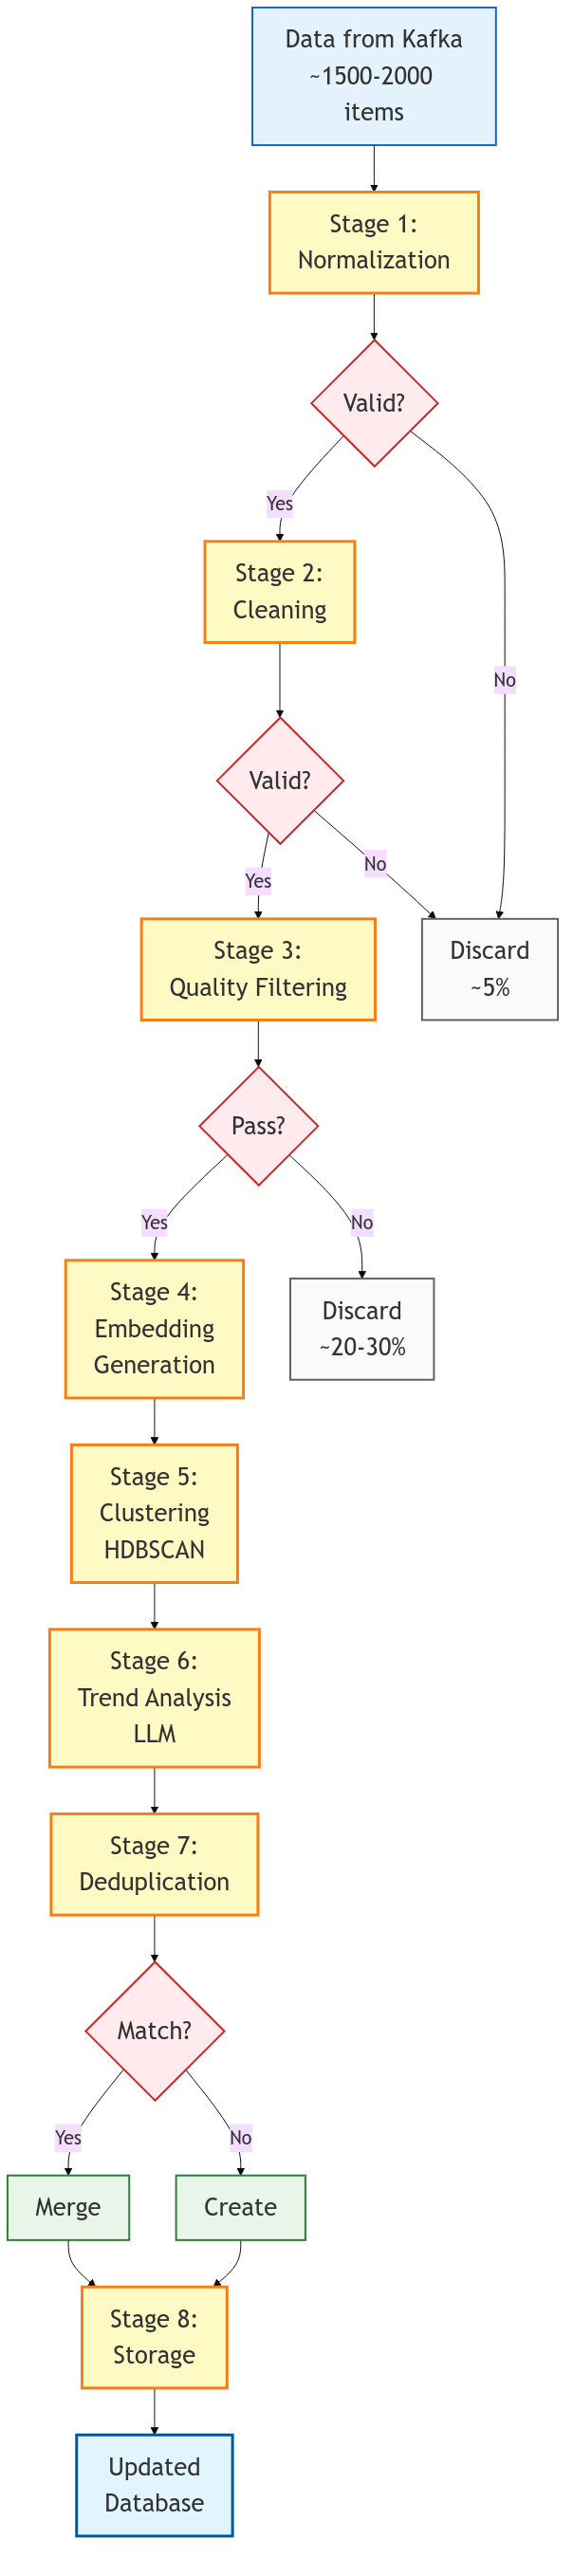
\includegraphics[width=0.3\textwidth]{images/pipeline.png}
    \caption{Sơ đồ chi tiết pipeline xử lý 8 giai đoạn}
    \label{fig:pipeline}
\end{figure}

\subsection{Cơ chế xử lý lỗi}

Hệ thống triển khai nhiều lớp xử lý lỗi để đảm bảo tính ổn định. Ở tầng Producer, nếu API call thất bại, hệ thống retry tối đa 3 lần với exponential backoff (1s, 2s, 4s). Nếu vẫn thất bại, skip source đó và tiếp tục các source khác. Ở tầng Consumer, nếu embedding API hoặc LLM API gặp rate limit, hệ thống tự động chờ và retry. Nếu xảy ra lỗi nghiêm trọng (crash, exception), Consumer không commit offset, đảm bảo dữ liệu sẽ được xử lý lại trong lần chạy tiếp theo.

Hệ thống ghi log chi tiết ở mọi giai đoạn, bao gồm: số lượng items ở mỗi stage, số lượng items bị loại bỏ, số cụm phát hiện, số trends mới/merged, và thời gian xử lý. Logs được lưu vào file và có thể xem qua Docker logs. Ngoài ra, hệ thống có health check endpoint để monitoring.

\section{Tầng giao diện (Dashboard)}

\subsection{User Dashboard}

User Dashboard được xây dựng bằng Streamlit, cung cấp giao diện web để người dùng xem và tìm kiếm xu hướng. Dashboard hiển thị danh sách xu hướng được sắp xếp theo tổng engagement (views + likes) giảm dần, đảm bảo xu hướng hot nhất xuất hiện đầu tiên.

Mỗi trend card hiển thị đầy đủ thông tin: topic (tiêu đề lớn), summary (tóm tắt nội dung), sentiment với màu sắc tương ứng (xanh lá - tích cực, đỏ - tiêu cực, xám - trung lập), risk\_level với icon cảnh báo, content\_type, keywords dạng tags, total stats (tổng views, likes, engagement rate), source distribution (biểu đồ phần trăm TikTok/YouTube/News), và top 5 sample videos với link trực tiếp.

Dashboard cung cấp các chức năng filter và search: (1) Text search - tìm kiếm theo topic hoặc keywords; (2) Sentiment filter - lọc theo cảm xúc (all/positive/negative/neutral); (3) Content type filter - lọc theo loại nội dung; (4) Risk level filter - lọc theo mức độ rủi ro. Bên cạnh đó, user có thể đề xuất từ khóa mới qua form, submission sẽ được lưu vào database với status 'pending' chờ admin duyệt.

\begin{figure}[H]
    \centering
    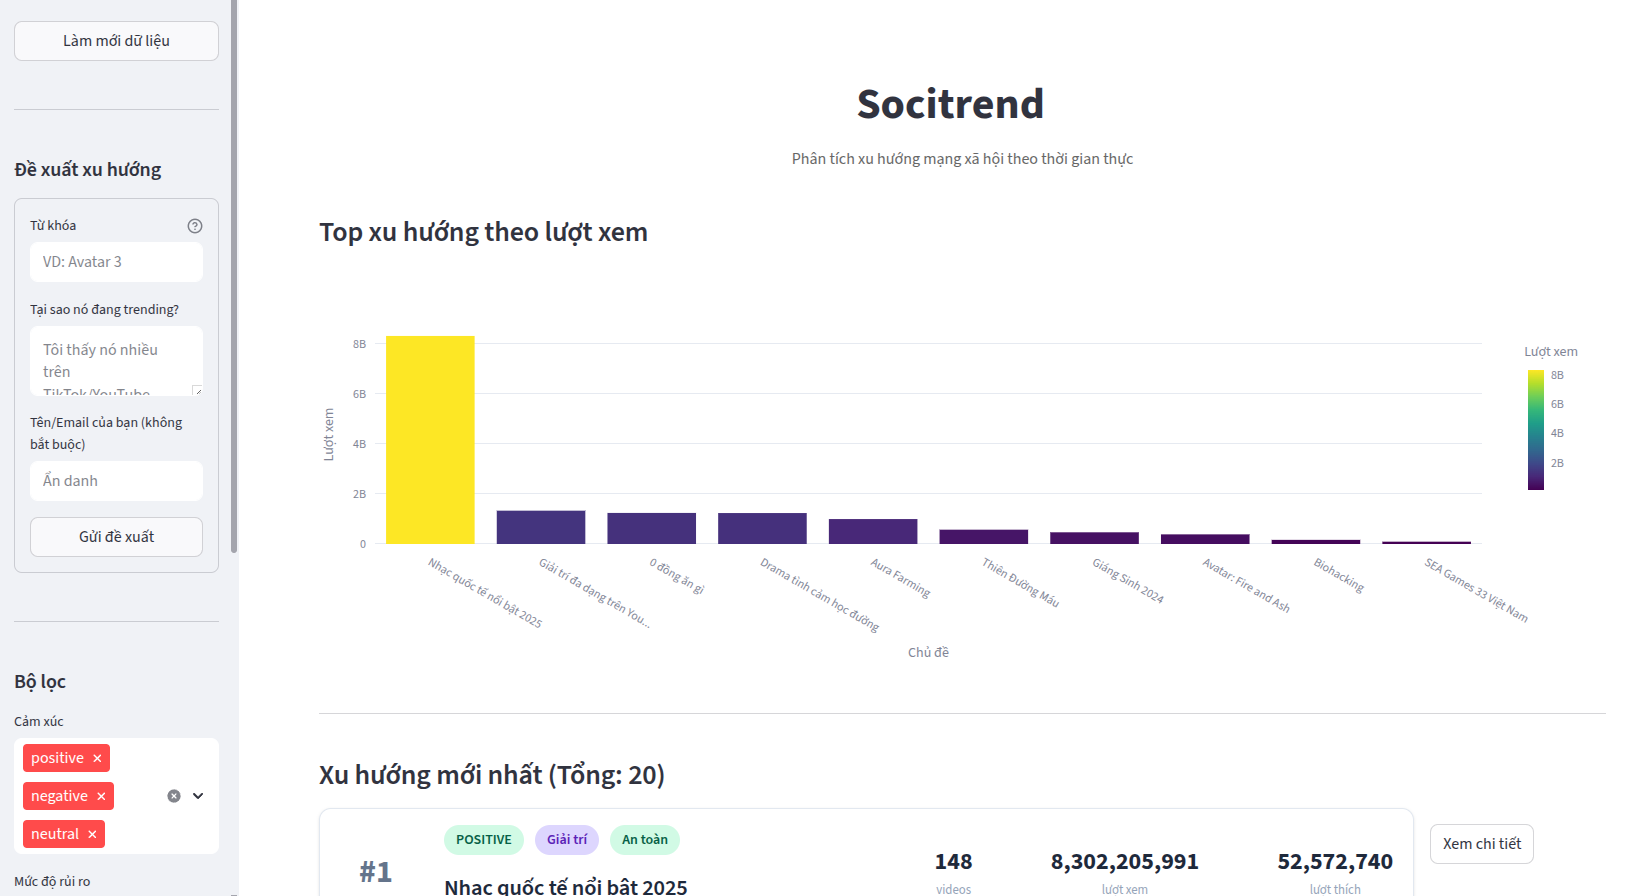
\includegraphics[width=\textwidth]{images/user.png}
    \caption{Giao diện User Dashboard hiển thị xu hướng và chức năng tìm kiếm}
    \label{fig:user-dashboard}
\end{figure}

\subsection{Admin Dashboard}

Admin Dashboard cung cấp các chức năng quản trị hệ thống. Giao diện chia thành ba tabs: Quản lý xu hướng, Đề xuất từ khóa, và Từ khóa hoạt động.

\textbf{Quản lý xu hướng:} Admin có thể xem tất cả trends với đầy đủ thông tin, tìm kiếm theo topic, và xóa trends không mong muốn. Mỗi trend hiển thị thêm thông tin kỹ thuật như trend\_id, created\_at, updated\_at. Chức năng xóa có confirmation để tránh xóa nhầm.

\textbf{Đề xuất từ khóa:} Tab này chia làm hai cột để quản lý từ khóa từ hai nguồn khác nhau. Cột trái hiển thị đề xuất từ người dùng (user submissions) với thông tin keyword, reason, submitted\_by, status. Admin có thể approve hoặc reject từng submission. Cột phải hiển thị từ khóa được Keyword Extractor tự động trích xuất từ tin tức, bao gồm keyword, category (giải trí/công nghệ/...), reason (lý do trending), status. Mỗi extracted keyword có button "Thêm vào keywords" để approve và tự động thêm vào active\_keywords áp dụng cho tất cả nguồn, hoặc "Bỏ qua" để reject. Cả hai nguồn đều có filter theo status (pending/approved/rejected/all) để dễ quản lý.

\textbf{Từ khóa hoạt động:} Hiển thị danh sách active\_keywords hiện tại với các chức năng: (1) Thêm keyword mới thủ công qua form; (2) Sửa keyword hiện có - khi click "Sửa", keyword chuyển thành input field với buttons "Lưu"/"Hủy", cho phép admin chỉnh sửa nhanh; (3) Xóa keyword không còn cần thiết. Tất cả thay đổi được ghi log vào keyword\_history collection để audit: action (add/update/remove/approve), keyword, performed\_by, timestamp, details (old\_keyword, new\_keyword). Mỗi keyword áp dụng cho tất cả ba nguồn TikTok, YouTube và News.

\begin{figure}[H]
    \centering
    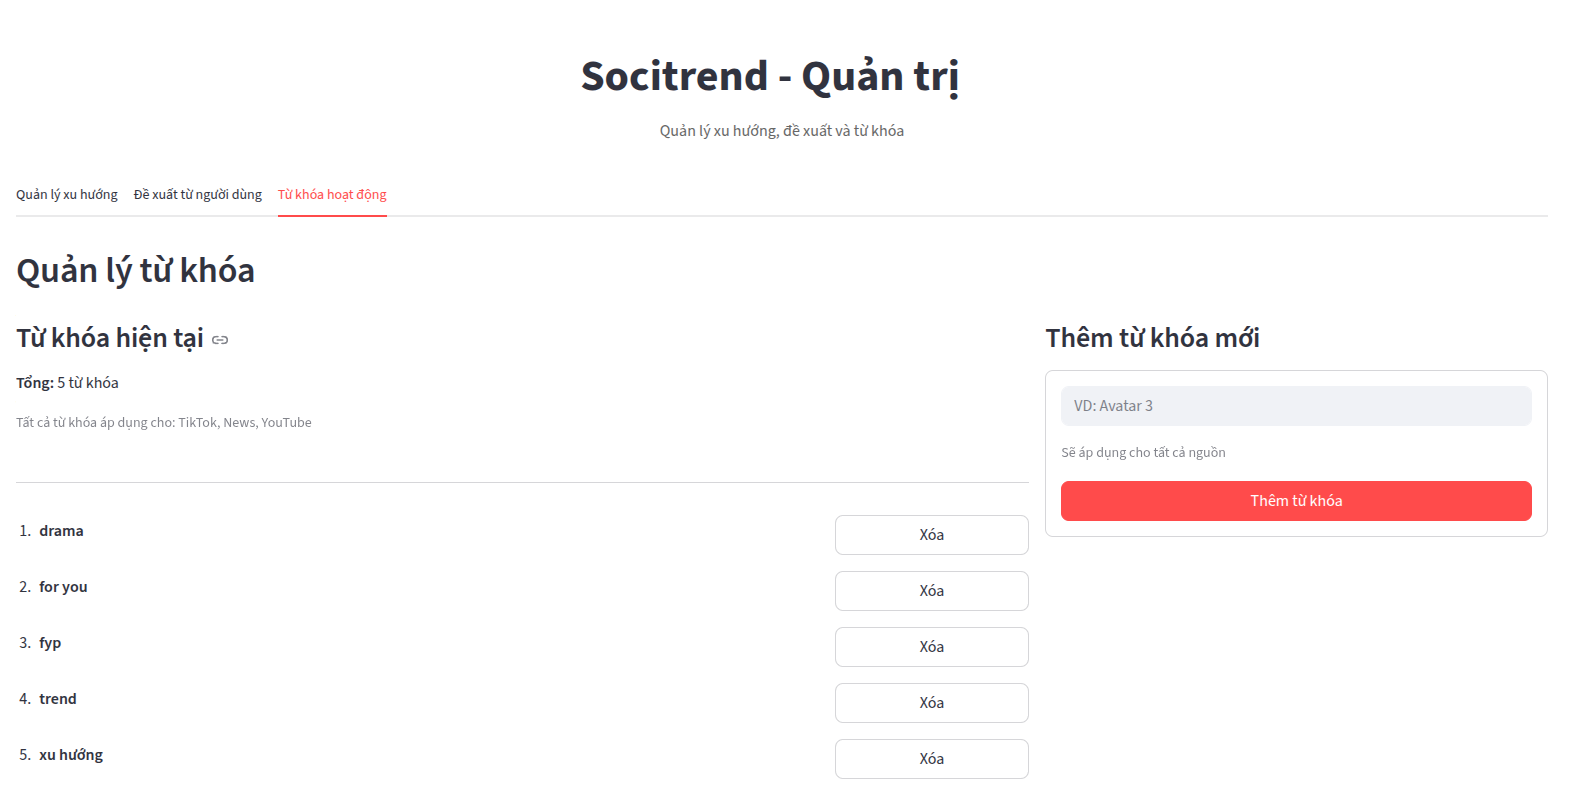
\includegraphics[width=\textwidth]{images/admin.png}
    \caption{Giao diện Admin Dashboard với các chức năng quản trị hệ thống}
    \label{fig:admin-dashboard}
\end{figure}

